\chapter{Inference using Nonlinear Hybrid Models}
In this section we study the same graphical model as Section \ref{sec_inf_lin_hybrid}, shown in Figure \ref{fig_hybridmod2} for convenience, but we drop the assumption that the dynamic models are linear. The variables retain their meaning as before.     
\begin{figure}[H] 
\centering
\begin{tikzpicture}

  % Define nodes
  \node[obs] (ya) {$y_0$};
  \node[obs, right=of ya] (yb) {$y_1$};
  \node[obs, right=of yb] (yc) {$y_2$};
  \node[latent, above=of ya]  (xa) {$x_0$};
  \node[latent, above=of yb, right=of xa]  (xb) {$x_1$};
  \node[latent, above=of yc, right=of xb]  (xc) {$x_2$};
  \node[det, above=of xa, xshift=0.7cm] (da) {$u_0$};
  \node[det, above=of xb, xshift=0.7cm] (db) {$u_1$};
  \node[latent, above=of xa, yshift=1.1cm] (sa) {$s_0$};
  \node[latent, above=of xb, yshift=1.1cm] (sb) {$s_1$};
  \node[latent, above=of xc, yshift=1.1cm] (sc) {$s_2$};
  
  % Connect the nodes
  \edge {da} {xb};
  \edge {db} {xc};
  \edge {xa} {ya};
  \edge {xb} {yb};
  \edge {xc} {yc};
  \edge {xa} {xb};
  \edge {xb} {xc};
  \edge {sa} {sb};
  \edge {sb} {sc};
  \edge {sa} {xa};
  \edge {sb} {xb};
  \edge {sc} {xc};
  
\end{tikzpicture}
\caption{Graphical model of this section}
\label{fig_hybridmod2}
\end{figure}
Intuitively we are now using the switching variables to decide which nonlinear model (or combination of) better describes the observed system behaviour. At each point in time we desire a weighted set of nonlinear models with the weight proportional to the ability of the model to explain the plant behaviour. Such a system could be used to describe significant model changes e.g. catalyst degradation in our CSTR or a reactor which breaks suddenly etc... 

We model this system as follows. Let $s_t \in (1,2,..., M)$ denote a discrete $M$ state first order Markov chain with transition matrix $P$ as discussed in Section \ref{sec_inf_lin_hybrid}. Let each state $s_t=i$ be associated with a model set $\left(f_i, g_i, W_i, V_i \right)$ used to evaluate the dynamical model shown in (\ref{eq_smodel2}).
\begin{equation}
\begin{aligned}
x_{t+1} &= f_i(x_t, u_t, w_{t+1}) \text{ with } w_{t+1} \backsim \mathcal{N}(0, W_i)\\
y_{t+1} &= g_i(x_{t+1}, v_{t+1}) \text{ with } v_{t+1} \backsim \mathcal{N}(0,V_i)
\end{aligned}
\label{eq_smodel2}
\end{equation}
In this dissertation we assume that the the noise distributions are Gaussian but there is no fundamental reason why they cannot be arbitrary. To fully specify the system we again require the prior distributions $p(s_0)$ and $p(x_0|s_0)$ as well as the stochastic matrix $P$. In this section we manually specify the matrix $P$ but it can be computed using the Baum-Welch Algorithm. 
\section{Exact Filtering}
By extending the model to incorporate nonlinear models it becomes even more difficult to perform inference. It is clear that for the type of systems we consider here no exact inference algorithm, which is computationally feasible, exists \cite{murphy1}. We again turn to approximate inference algorithms.

Note that we cannot apply Rao-Blackwellisation (i.e. analytically evaluate the stochastic dynamical system component and approximate the switching component) as before because the dynamic models are no longer linear. We use the adaptive Sequential Importance Resampling, i.e. the bootstrap Particle Filter, algorithm as discussed in Section \ref{sec_inf_nonlin_mods}.
\section{Switching Particle Filter}
We cannot analytically evaluate any part of the desired posterior distribution $p(s_{0:t}, x_{0:t}|y_{0:t})$ in a computationally feasible manner, so we must apply the adaptive Sequential Importance Resampling algorithm to the entire state space of Figure \ref{fig_hybridmod2}. The algorithm follows straightforwardly from our discussion in Section \ref{sec_asir} \cite{murphy1}. We merely state the incremental weight function and proposal distribution we sample from in (\ref{eq_nonpf}). 
\begin{equation}
\begin{aligned}
&q_t(s_t,x_t|s_{0:t-1},x_{0:t-1,}y_{0:t}) = p(s_t|s_{t-1})p(x_t|s_t,x_{t-1}) \\
&\alpha_t(s_{0:t},x_{0:t}) = p(y_t|x_t,s_t)
\end{aligned}
\label{eq_nonpf}
\end{equation}  
Applying the algorithm is a straightforward extension of the bootstrap Particle Filter introduced in Section \ref{sec_bootstrap} given the weighting function and proposal distribution as shown below.

\textbf{Switching Particle Filter Algorithm}\\
For $t=0$:
\begin{enumerate}
\item
Sample $S^i_0 \backsim p(s_0)$ and $X^i_0 \backsim p(x_0|s_0)$.
\item
Compute the weights $w_0(S_0^i, X_0^i) = p(y_0|S_0^i, X_0^i)$ where $y_0$ is the observation. Normalise $W^i_0 \propto w_0(S_0^i, X_0^i)$. 
\item
If the number of effective particles is below some threshold apply resampling with roughening $(W^i_0, S^i_0, X^i_0)$ to obtain $N$ equally weighted particles $(\frac{1}{N}, \bar{S}^i_0, \bar{X}^i_0)$ and set $(\bar{W}^i_0, \bar{S}^i_0,\bar{X}^i_0) \leftarrow (\frac{1}{N}, \bar{S}^i_0, \bar{X}^i_0)$ otherwise set $(\bar{W}^i_0,\bar{S}^i_0, \bar{X}^i_0) \leftarrow ({W}^i_0, S_0^i, {X}^i_0)$
\end{enumerate}
For $t \geq 1$:
\begin{enumerate}
\item
Sample $S^i_t \backsim p(S_t^i|\bar{S}^i_{t-1})$ and $X^i_t \backsim p(X^i_t|S^i_t, \bar{X}^i_{t-1})$.
\item
Compute the weights $\alpha_t(S_t^i, X_t^i) = p(y_t|S_t^i, X_t^i)$ where $y_t$ is the observation. Normalise $W^i_t \propto W^i_{t-1}\alpha_t(S_t^i, X_t^i)$.
\item
If the number of effective particles is below some threshold apply resampling with roughening $(W^i_t, S^i_t, X^i_t)$ to obtain $N$ equally weighted particles $(\frac{1}{N}, \bar{S}^i_t, \bar{X}^i_t)$ and set $(\bar{W}^i_t, \bar{S}^i_t,\bar{X}^i_t) \leftarrow (\frac{1}{N}, \bar{S}^i_t, \bar{X}^i_t)$ otherwise set $(\bar{W}^i_t,\bar{S}^i_t, \bar{X}^i_t) \leftarrow ({W}^i_t, S_t^i, {X}^i_t)$
\end{enumerate} 

\section{Switching Particle Prediction}
The prediction of the hybrid non-linear states follows in an analogous manner to the prediction algorithm found in Section \ref{sec_particle_prediction}. We do not supply an algorithm because it is a straightforward simplification of the Switching Particle Filter algorithm seen above: effectively there is no weight update step because there is no observation. The corresponding Graphical Model is shown in Figure \ref{fig_hybridmod2_prediction}.
\begin{figure}[H] 
\centering
\begin{tikzpicture}

  % Define nodes
  \node[obs] (ya) {$y_0$};
  \node[latent, above=of ya]  (xa) {$x_0$};
  \node[latent, above=of yb, right=of xa]  (xb) {$x_1$};
  \node[latent, above=of yc, right=of xb]  (xc) {$x_2$};
  \node[det, above=of xa, xshift=0.7cm] (da) {$u_0$};
  \node[det, above=of xb, xshift=0.7cm] (db) {$u_1$};
  \node[latent, above=of xa, yshift=1.1cm] (sa) {$s_0$};
  \node[latent, above=of xb, yshift=1.1cm] (sb) {$s_1$};
  \node[latent, above=of xc, yshift=1.1cm] (sc) {$s_2$};
  
  % Connect the nodes
  \edge {da} {xb};
  \edge {db} {xc};
  \edge {xa} {ya};
  \edge {xa} {xb};
  \edge {xb} {xc};
  \edge {sa} {sb};
  \edge {sb} {sc};
  \edge {sa} {xa};
  \edge {sb} {xb};
  \edge {sc} {xc};
  
\end{tikzpicture}
\caption{Switching Particle Prediction Graphical Model}
\label{fig_hybridmod2_prediction}
\end{figure}  

\section{Smoothing and Viterbi Decoding}
Like Section \ref{sec_inf_lin_hybrid} we refer the reader elsewhere for a detailed discussion on both smoothing and Viterbi Decoding \cite{murphy1}. It suffices to say that given the non-linear dynamics the aforementioned inference will be beyond the scope of this dissertation. 

\section{Filtering the CSTR}
In this section we illustrate the use of the Switching Particle Filter (SPF) using  two non-linear dynamical model derived from the familiar CSTR example of Section \ref{sec_cstr}. Since the Graphical Model of Section \ref{sec_inf_lin_hybrid} is identical to that of Figure \ref{fig_hybridmod2} we expect, and assume, that the general trends discussed in Section \ref{sec_rbpf_filtering_cstr} to hold here as well.

For the purposes of illustration we assume a scenario where the rate constant of the CSTR decreases by an order of magnitude. This scenario is not completely arbitrary, for example, this could be caused by catalyst degradation due to some environmental factor. It is our aim to infer when this happens and to be able to track the states accurately despite the significant model change. Therefore we will have one non-linear model of the healthy plant $M_1$ and one non-linear model of the faulty plant $M_2$. 

We use 500 particles during all runs for the SPF and use the switching transition matrix $P=\begin{pmatrix}
0.99 & 0.01 \\ 0.01 & 0.99
\end{pmatrix}$. For the Particle Filter we use 200 particles. We spent much time in Section \ref{sec_rbpf_filtering_cstr} discussing the effect the switch transition matrix has on model selection. The form of the matrix is motivated by physical considerations as well: once the catalyst denatures it is unlikely to fix itself. Thus, once the model breaks, switches to $M_2$ from $M_1$ it is unlikely to switch back. In all the simulations the catalyst denatures at 50 minutes into the run.

We conduct two brief but illustrative investigations comparing the effectiveness of the SPF to the Particle Filter (PF). In both cases the PF uses the healthy system model - the benefit of the SPF is highlighted here. In the first investigation we measure only temperature and in the second we measure both concentration and temperature. 

In Figure \ref{fig_pf_m1_compspf} we illustrate the tracking performance of the PF on the system. Note that the simulation window is very long - 600 minutes.
\begin{figure}[H] 
\centering
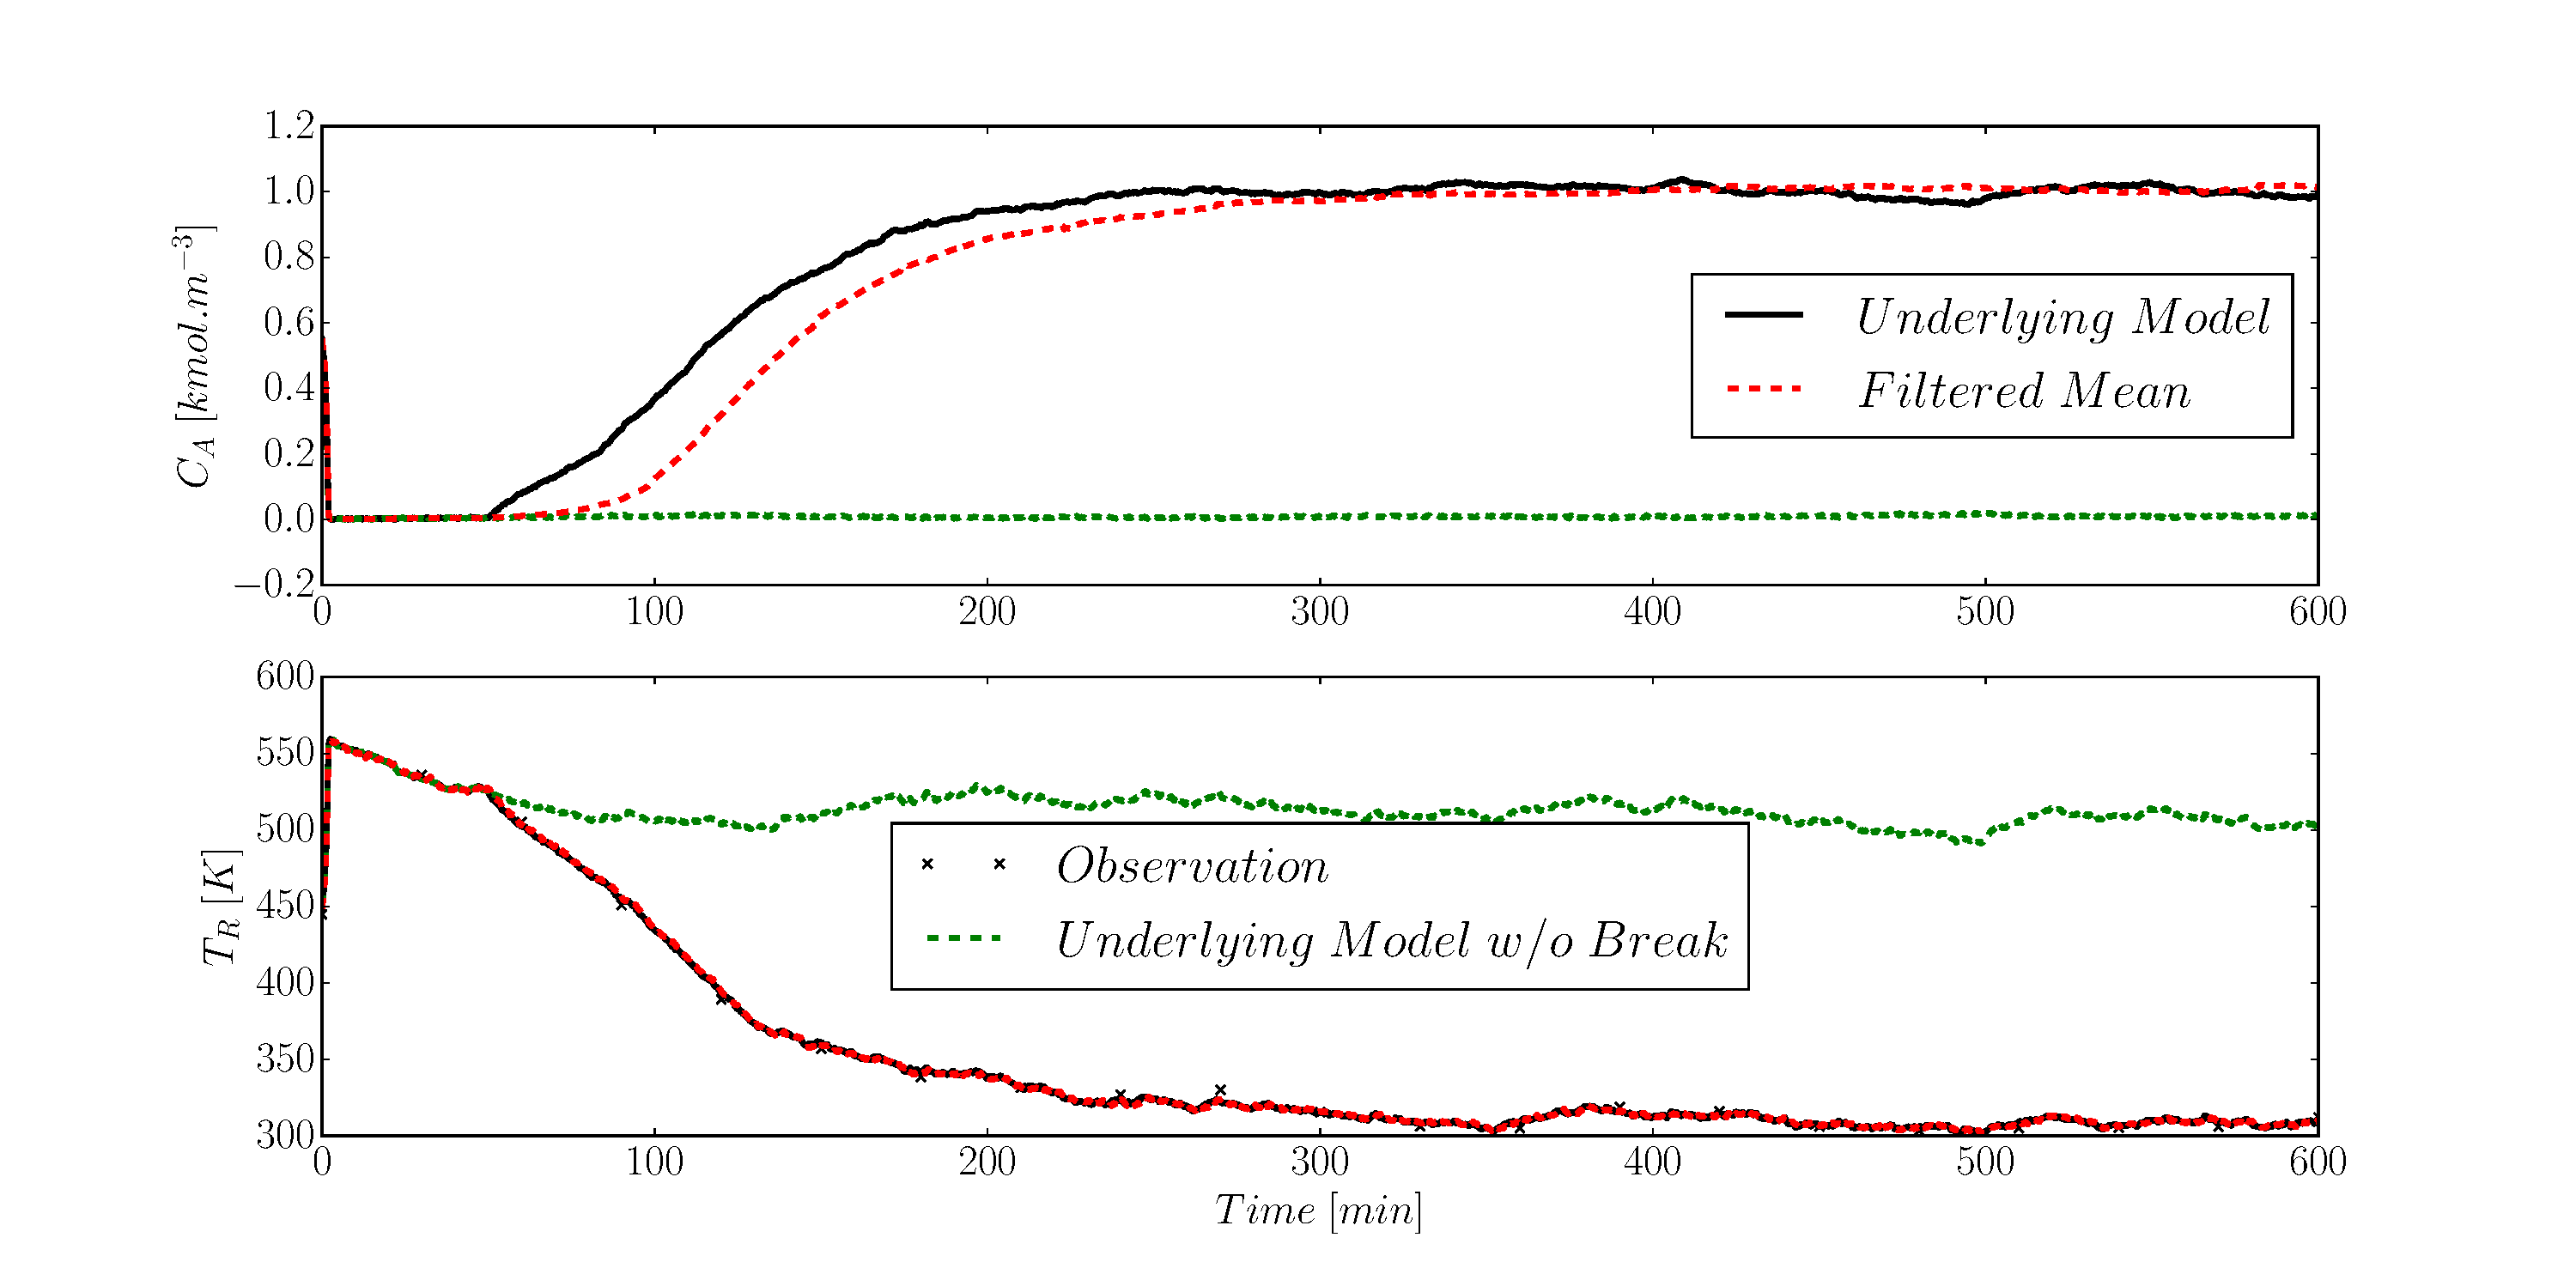
\includegraphics[scale=0.3]{pf_m1_compspf.pdf}
\caption{Particle Filter using 200 particles tracking the CSTR where the catalyst denatures at 50 minutes.}
\label{fig_pf_m1_compspf}
\end{figure}
It is clear that the PF tracks the temperature well, because it is measured, but tracks the concentration very poorly. It takes almost 300 minutes before the PF estimates the concentration somewhat reliably. Clearly the model mismatch causes the filter's poor performance.

In Figure \ref{fig_spf_m1_track}
\begin{figure}[H] 
\centering
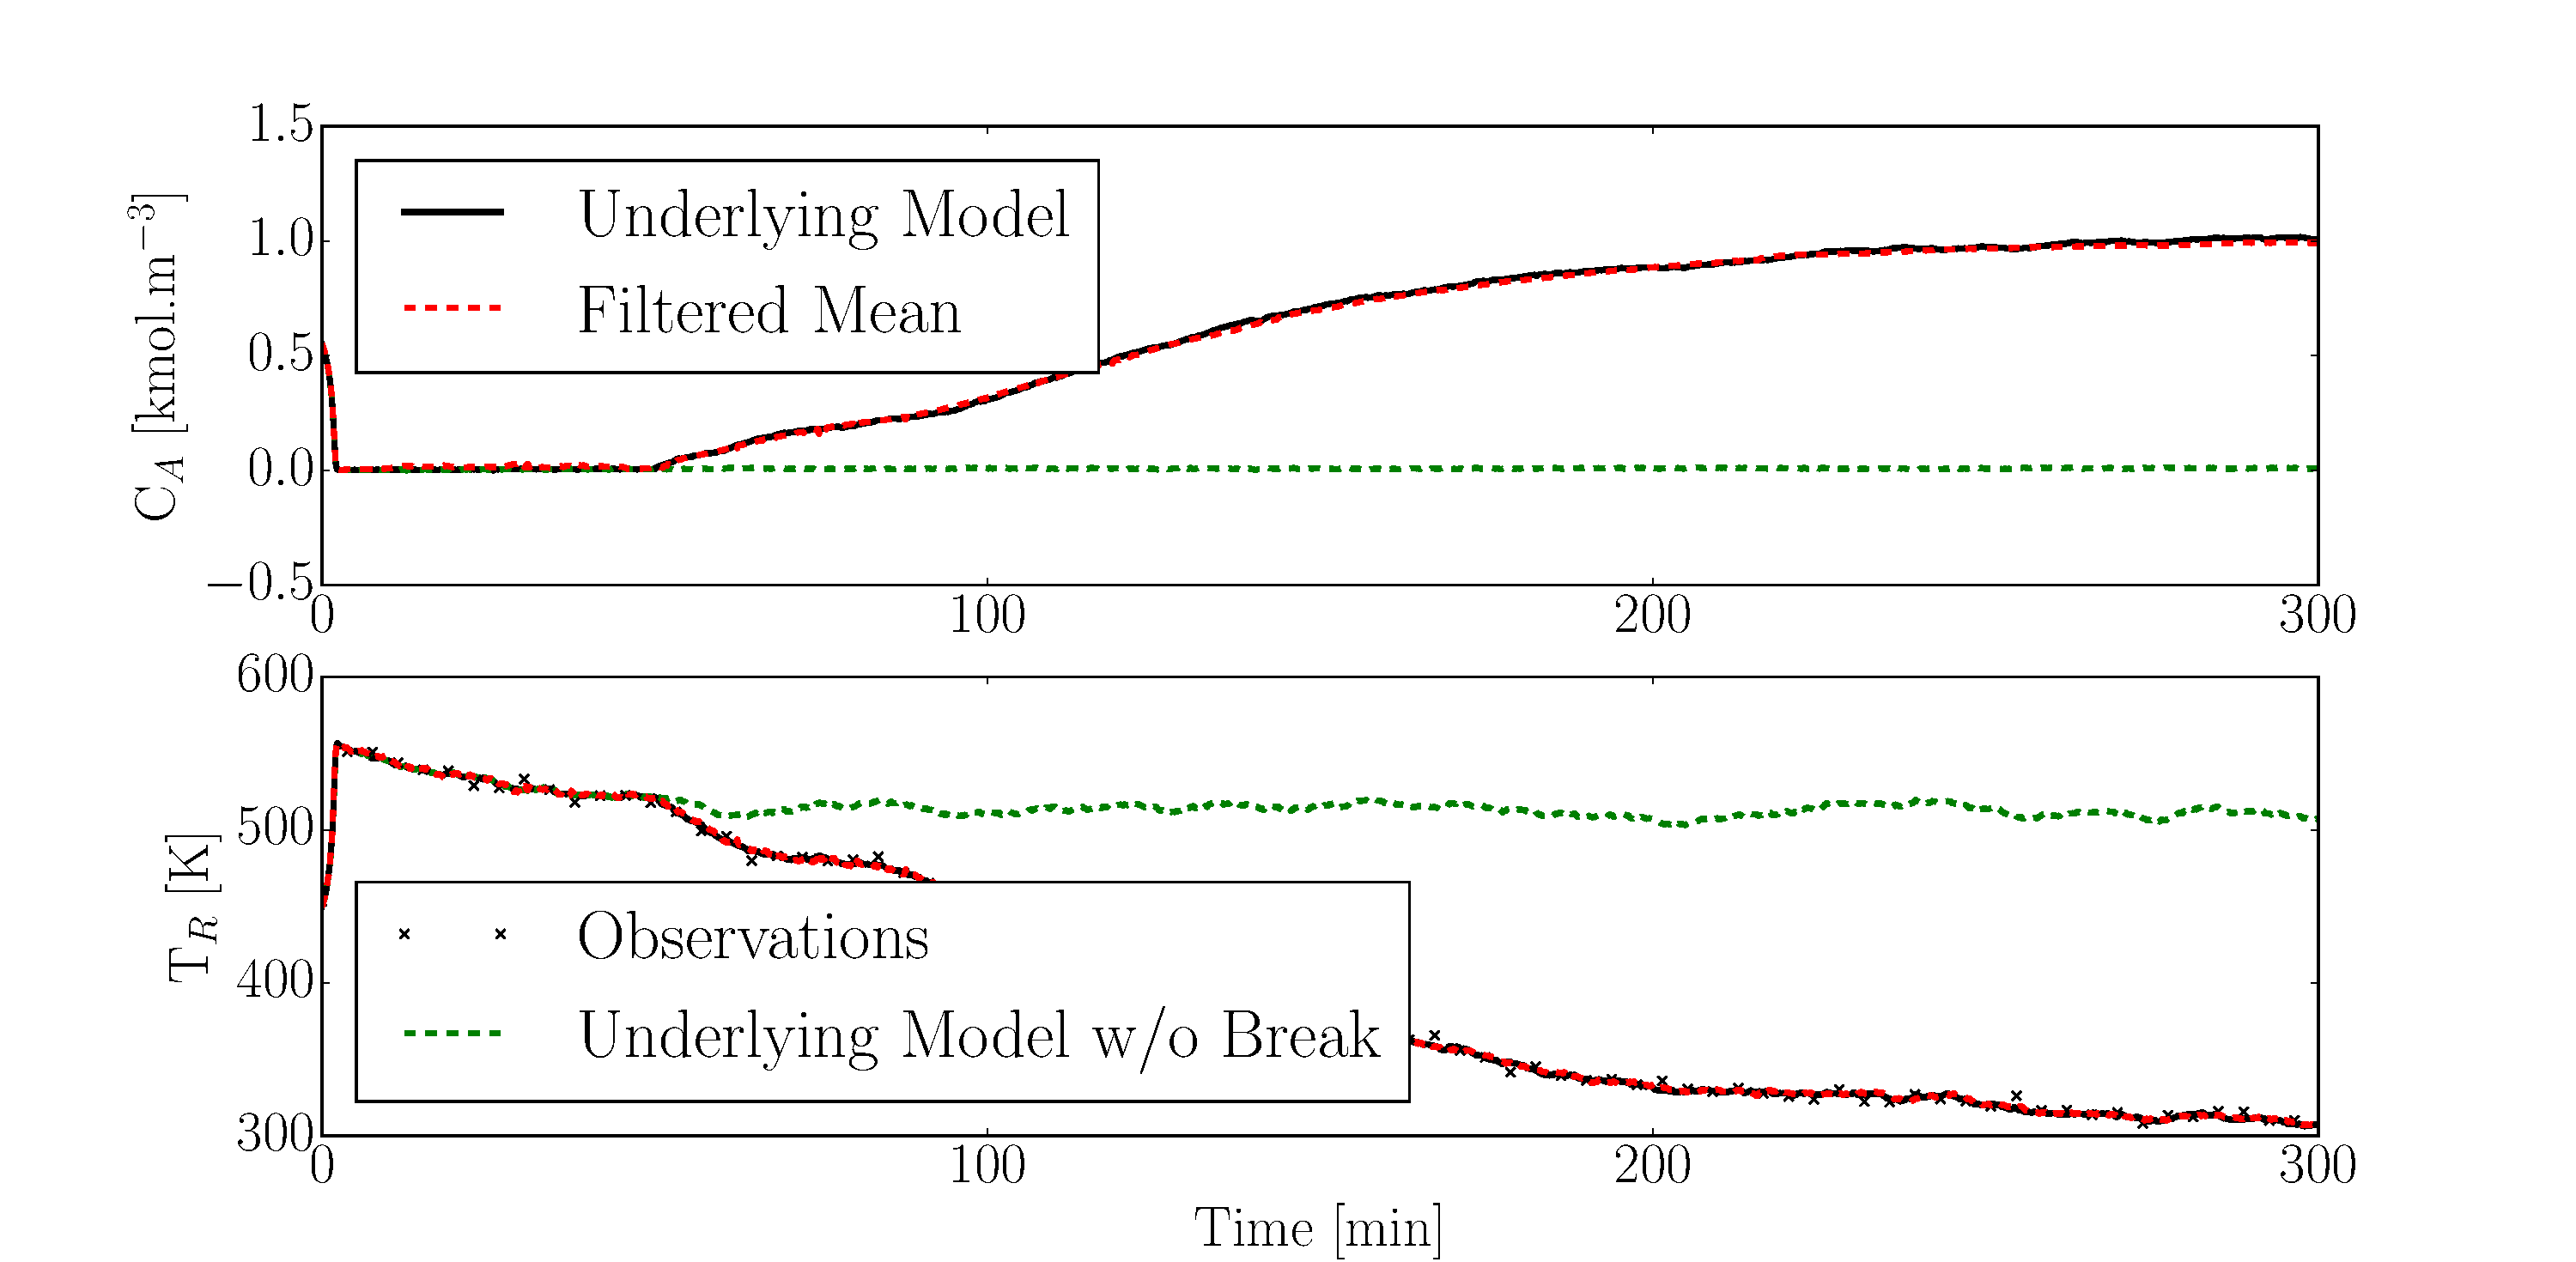
\includegraphics[scale=0.3]{spf_m1_track.pdf}
\caption{Switching Particle Filter using 500 particles tracking the CSTR where the catalyst denatures at 50 minutes.}
\label{fig_spf_m1_track}
\end{figure}

\begin{figure}[H] 
\centering
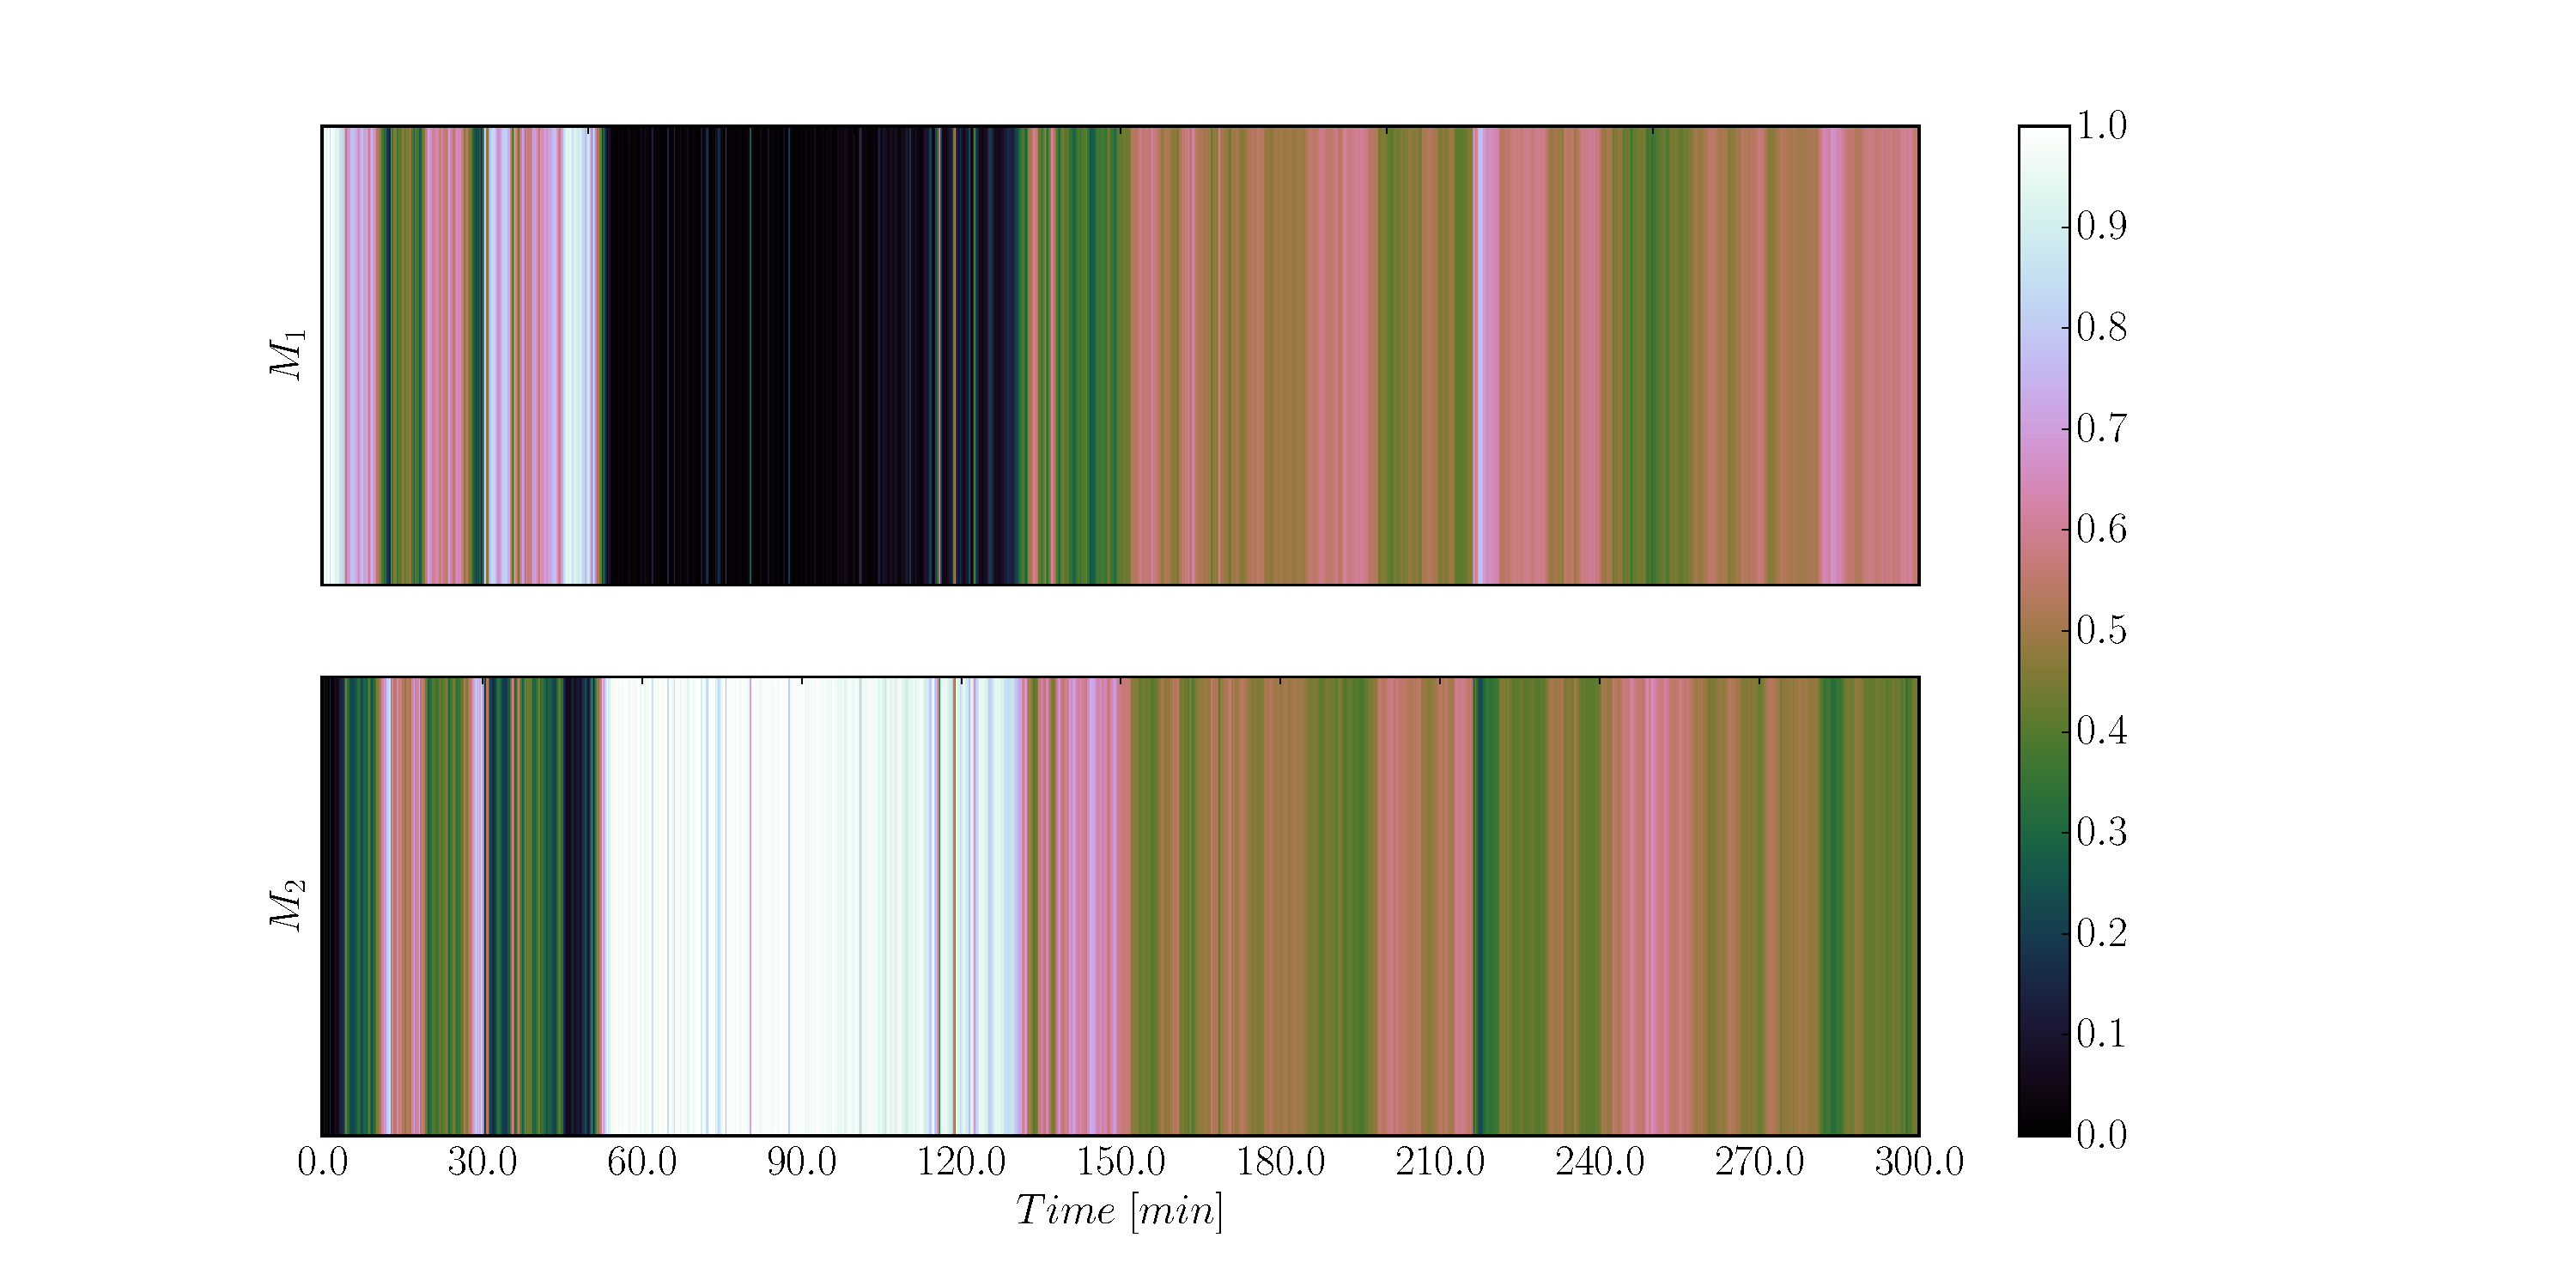
\includegraphics[scale=0.3]{spf_m1_switch.pdf}
\caption{Switching Particle Filter measuring only temperature. The switching weight of each particle is shown per time step.}
\label{fig_spf_m1_switch}
\end{figure} 